% Wersja źródłowa: audyt II, jednostka 18
\setcounter{section}{1}
\section{Funkcje testowe i ścisłe granice induktywne}
\label{sec:funkcje-testowe18}

\providecommand{\atlasref}[2]{#2}


\subsection{Funkcje o ustalonym zwartym nośniku}

\noindent\emph{Powiązania tematyczne w Bibliotece matematycznej:} \atlasref{PDE-07::def:pde7-test}{PDE-07: funkcje testowe}.


W całym rozdziale zakładamy, że $d\ge1$ jest liczbą całkowitą,
$\Omega\subseteq\R^d$ jest niepustym zbiorem otwartym,
a $\K\in\{\R,\C\}$. Oznaczenia wielowskaźników i seminorm
$p_{K,m}$ przyjmujemy jak w rozdziale~\ref{sec:gladkie-schwartz17}.
Dla $f\in C^\infty(\Omega;\K)$ definiujemy jego \emph{nośnik}
przez $\supp f=\overline{\{x\in\Omega:f(x)\ne0\}}^{\,\Omega}$,
tj. domknięcie względne w $\Omega$. Zapis $K\Subset\Omega$
oznacza, że $K$ jest zwartym podzbiorem $\Omega$.

\begin{definicja}[Przestrzeń $\mathcal D_K(\Omega)$]
\label{def:DK18}
Dla każdego zwartego $K\Subset\Omega$ kładziemy
\[
 \mathcal D_K(\Omega;\K)=\{\varphi\in C^\infty(\Omega;\K):
 \supp\varphi\subseteq K\}.
\]
Wyposażamy tę przestrzeń w topologię wyznaczoną przez seminormy
\[p_m(\varphi)=\max_{|\alpha|\le m}\sup_{x\in\Omega}
|\partial^\alpha\varphi(x)|,\qquad m\in\N_0.\]
Supremum jest skończone: na otwartym zbiorze $\Omega\setminus K$
funkcja i wszystkie jej pochodne znikają, a na $K$ są ciągłe
i ograniczone. Jeśli $K=\varnothing$, to $\mathcal D_K=\{0\}$.
Również gdy $\operatorname{int}K=\varnothing$, mamy
$\mathcal D_K=\{0\}$: dla niezerowej funkcji $\varphi$
zbiór $\{x\in\Omega:\varphi(x)\ne0\}$ jest niepusty,
otwarty i zawarty w $K$, co przeczy pustemu wnętrzu.
\end{definicja}

\begin{twierdzenie}[Struktura etapów]
\label{thm:DK-frechet18}
Dla każdego zwartego $K\Subset\Omega$ przestrzeń
$\mathcal D_K(\Omega;\K)$ jest przestrzenią Fr\'echeta.
Jeżeli $K\subseteq L\Subset\Omega$ są zwarte, to
$\mathcal D_K$ jest domkniętą podprzestrzenią $\mathcal D_L$,
a włożenie $\mathcal D_K\hookrightarrow\mathcal D_L$
jest izomorfizmem na swój obraz z topologią względną.
\end{twierdzenie}
\begin{proof}
Na mocy Twierdzenia~\ref{thm:frechet-cinf17}
$C^\infty(\Omega;\K)$ jest przestrzenią Frécheta.
Dla $x\in\Omega$ ewaluacja $\varphi\mapsto\varphi(x)$
jest ciągła, gdyż $|\varphi(x)|\le p_{\{x\},0}(\varphi)$.
Ponieważ $K$ jest domknięty w $\Omega$, mamy
\[
\mathcal D_K=\bigcap_{x\in\Omega\setminus K}
\ker(\varphi\mapsto\varphi(x)).
\]
Jest to przecięcie domkniętych podprzestrzeni liniowych,
a więc domknięta podprzestrzeń $C^\infty(\Omega;\K)$.
Dla każdego zwartego $L\Subset\Omega$ oraz $m\in\N_0$
na $\mathcal D_K$ mamy $p_{L,m}\le p_m$.
Z drugiej strony $p_m=p_{K,m}$ na $\mathcal D_K$,
gdyż wszystkie pochodne znikają poza $K$
(dla pustego $K$ obie seminormy są zerowe).
Obie rodziny wyznaczają zatem tę samą topologię.
Domknięta podprzestrzeń przestrzeni Fr\'echeta jest przestrzenią
Fr\'echeta. Ten sam argument, zastosowany do $K\subseteq L$,
daje domkniętość $\mathcal D_K$ w $\mathcal D_L$;
seminormy $p_m$ są na obu etapach określone tym samym wzorem.
\end{proof}

\begin{definicja}[Algebraiczna przestrzeń funkcji testowych]
\label{def:D-algebraic18}
Oznaczamy przez $\mathcal D(\Omega;\K)=C_c^\infty(\Omega;\K)$
przestrzeń wszystkich funkcji gładkich o zwartym nośniku.
Jeśli $(K_n)_{n\ge1}$ jest wyczerpaniem zwartymi zbiorami,
$K_n\subseteq\operatorname{int}K_{n+1}$ i każdy zwarty
$K\Subset\Omega$ jest zawarty w pewnym $K_n$, to
$\mathcal D(\Omega)=\bigcup_{n\ge1}\mathcal D_{K_n}(\Omega)$.
Takie wyczerpanie skonstruowano w Lemacie~\ref{lem:exhaustion17}.
Równość wynika stąd, że nośnik każdej funkcji testowej
jest zawarty w pewnym $K_n$, a każda funkcja z $\mathcal D_{K_n}$
ma zwarty nośnik.
\end{definicja}

\subsection{Topologia granicy induktywnej}

\noindent\emph{Powiązania tematyczne w Bibliotece matematycznej:} \atlasref{KAT-08::def:colimit}{KAT-08: kogranice i ich własność uniwersalna (właściwa kategoria ma tu znaczenie)}; \atlasref{GT-04::thm:topog-koncowa-uniwersalnosc}{GT-04: topologia końcowa (porównanie z granicą induktywną lokalnie wypukłą)}.


\begin{definicja}[Lokalnie wypukła granica induktywna]
\label{def:LF18}
Niech $(E_n,\tau_n)_{n\ge1}$ będzie ciągiem przestrzeni
lokalnie wypukłych nad tym samym ciałem $\K\in\{\R,\C\}$,
przy czym $E_n\subseteq E_{n+1}$ jako przestrzenie liniowe
i każde włożenie
$i_n:E_n\hookrightarrow E_{n+1}$ jest liniowe i ciągłe.
Na $E=\bigcup_nE_n$ rozważamy \emph{najsilniejszą lokalnie
wypukłą topologię}, dla której wszystkie odwzorowania
$E_n\hookrightarrow E$ są ciągłe. Oznaczamy ją
$\operatorname{ind}_n E_n$ i nazywamy topologią granicy induktywnej.
Na etapie ogólnej konstrukcji dopuszczamy topologię,
która nie musi spełniać warunku Hausdorffa.
Warunek ten zachodzi wtedy i tylko wtedy, gdy ciągłe
seminormy granicy oddzielają punkty. Jeśli $E_n$ są
przestrzeniami Frécheta i granica jest Hausdorffa,
nazywamy ją przestrzenią typu $(LF)$.
Granica jest \emph{ścisła}, jeśli
każde $E_n$ ma topologię względną z $E_{n+1}$ i jest w nim
podprzestrzenią domkniętą.
\end{definicja}

\begin{twierdzenie}[Konstrukcja przez seminormy i własność uniwersalna]
\label{thm:LF-universal18}
Niech $(E_n,\tau_n)_{n\ge1}$ będzie rosnącym ciągiem
przestrzeni lokalnie wypukłych nad tym samym ciałem $\K$,
z ciągłymi włożeniami liniowymi, a $E=\bigcup_{n\ge1}E_n$
niech będzie wyposażona w topologię granicy induktywnej
z Definicji~\ref{def:LF18}. Rozważmy rodzinę
$\mathcal P$ wszystkich seminorm $p:E\to[0,\infty)$ takich,
że $p|_{E_n}$ jest ciągła dla każdego $n$.
Topologia generowana przez $\mathcal P$ jest topologią
granicy induktywnej. Dla dowolnej przestrzeni lokalnie
wypukłej $F$ i odwzorowania liniowego $T:E\to F$ mamy
\[
 T\text{ jest ciągłe}\quad\Longleftrightarrow\quad
 T|_{E_n}:E_n\to F\text{ jest ciągłe dla każdego }n.
\]
\end{twierdzenie}
\begin{proof}
Oznaczmy przez $\tau_{\mathcal P}$ topologię wyznaczoną przez
$\mathcal P$. Przeciwobraz podstawowego otoczenia zera
$\bigcap_{j=1}^r\{x\in E:p_j(x)<\varepsilon_j\}$
przez włożenie $E_n\hookrightarrow E$ jest przecięciem
otoczeń zera określonych przez ciągłe seminormy $p_j|_{E_n}$.
Włożenie jest zatem ciągłe w topologii $\tau_{\mathcal P}$. Niech $\rho$ będzie
inną lokalnie wypukłą topologią na $E$, dla której włożenia
są ciągłe. Każda seminorma ciągła dla $\rho$ należy do
$\mathcal P$, gdyż jej ograniczenie do $E_n$ jest ciągłe.
Stąd $\rho$ jest nie silniejsza od naszej topologii.
Jeśli $T$ jest ciągłe, to każde $T|_{E_n}$ jest ciągłe
jako złożenie z ciągłym włożeniem.
Odwrotnie, niech wszystkie $T|_{E_n}$ będą ciągłe.
Dla każdej ciągłej seminormy $q$ na $F$ funkcja $q\circ T$
jest seminormą na $E$ dzięki liniowości $T$.
Jej ograniczenie do $E_n$ jest ciągłe, ponieważ jest równe
$q\circ(T|_{E_n})$. Zatem $q\circ T\in\mathcal P$,
a więc jest ciągła na $E$. Ponieważ ciągłe seminormy $q$
wyznaczają topologię $F$, ciągłość wszystkich $q\circ T$
daje ciągłość $T$.
\end{proof}

\begin{definicja}[Standardowa topologia $\mathcal D(\Omega)$]
\label{def:D-LF18}
Na $\mathcal D(\Omega;\K)$ przyjmujemy topologię
\[
 \mathcal D(\Omega;\K)
   =\operatorname{ind}_{n\to\infty}\mathcal D_{K_n}(\Omega;\K),
\]
gdzie $(K_n)$ jest wyczerpaniem z
Definicji~\ref{def:D-algebraic18}. Jest to \emph{standardowa
topologia funkcji testowych}. Nie należy jej utożsamiać
ani z topologią podprzestrzeni dziedziczoną po
$C^\infty(\Omega)$, ani automatycznie z końcową topologią
w kategorii wszystkich przestrzeni topologicznych.
\end{definicja}

\begin{stwierdzenie}[Niezależność od wyczerpania]
\label{prop:D-independence18}
Dla niepustego otwartego $\Omega\subseteq\R^d$ dwa rosnące
wyczerpania $\Omega$ zbiorami zwartymi, współkońcowe
wśród zwartych podzbiorów $\Omega$ prowadzą do tej samej
topologii na $\mathcal D(\Omega)$, nawet jeśli nie mają
identycznych wyrazów.
\end{stwierdzenie}
\begin{proof}
Niech $(K_n)$, $(L_j)$ będą takimi wyczerpaniami.
Seminorma $p$ na $\mathcal D(\Omega)$ jest ciągła na
każdym $\mathcal D_{K_n}$ wtedy i tylko wtedy, gdy jest
ciągła na każdym $\mathcal D_{L_j}$: dla ustalonego $K_n$
istnieje $L_j$ zawierający $K_n$, a ograniczenie seminormy
ciągłej na $\mathcal D_{L_j}$ do $\mathcal D_{K_n}$ jest
ciągłe. W drugą stronę argument jest symetryczny.
Korzystamy z Twierdzenia~\ref{thm:LF-universal18}.
\end{proof}

\begin{twierdzenie}[Topologia na każdym etapie i oddzielanie punktów]
\label{thm:D-stage18}
Dla dowolnego zwartego $K\Subset\Omega$ topologia względna
indukowana na $\mathcal D_K$ przez $\mathcal D(\Omega)$
jest topologią jego przestrzeni Fr\'echeta.
Ponadto $\mathcal D(\Omega)$ jest lokalnie wypukłą
przestrzenią liniowo-topologiczną Hausdorffa.
\end{twierdzenie}
\begin{proof}
Dla dowolnego zwartego $K\Subset\Omega$ wybieramy $n$
takie, że $K\subseteq K_n$. Włożenie $\mathcal D_K\to\mathcal D$
jest złożeniem dwóch ciągłych włożeń
$\mathcal D_K\to\mathcal D_{K_n}$ oraz
$\mathcal D_{K_n}\to\mathcal D$. Jego ciągłość oznacza, że
topologia względna nie jest silniejsza od topologii
$\mathcal D_K$. Dla każdego $m\in\N_0$ określmy na
całej $\mathcal D$ seminormę
$p_m(\varphi)=\max_{|\alpha|\le m}\sup_{x\in\Omega}
|\partial^\alpha\varphi(x)|$. Jej ograniczenie do
każdego $\mathcal D_{K_n}$ jest ciągłe, a zatem $p_m$
jest ciągła na $\mathcal D$ z
Twierdzenia~\ref{thm:LF-universal18}. Seminormy te
po ograniczeniu do $\mathcal D_K$ wyznaczają jego wyjściową
topologię Frécheta. Ponieważ są ciągłe w topologii względnej
indukowanej przez $\mathcal D$, topologia wyjściowa nie
jest od niej silniejsza. Obie topologie są więc równe.
Ponieważ $p_0(\varphi)>0$ dla $\varphi\ne0$, topologia
jest Hausdorffa; lokalna wypukłość wynika z konstrukcji.
Etapy $\mathcal D_{K_n}$ są przestrzeniami Frécheta
i są domkniętymi podprzestrzeniami kolejnych etapów
na mocy Twierdzenia~\ref{thm:DK-frechet18}.
Wobec tego $\mathcal D(\Omega;\K)$ jest ścisłą przestrzenią
typu $(LF)$ w sensie Definicji~\ref{def:LF18}.
\end{proof}

\begin{uwaga}[Przestrzeń dualna topologiczna]
\label{rem:D-dual18}
Własność uniwersalna jest szczególnie użyteczna dla
funkcjonałów: odwzorowanie liniowe $T:\mathcal D(\Omega)\to\K$
jest ciągłe wtedy i tylko wtedy, gdy każde ograniczenie
$T|_{\mathcal D_K}$ jest ciągłe. Ponieważ $\mathcal D_K$
ma topologię seminorm $p_m$, równoważnie: dla każdego
$K\Subset\Omega$ istnieją $C_K>0$ i $m_K\in\N_0$ takie, że
\[
 |T(\varphi)|\le C_K p_{m_K}(\varphi)
 \qquad(\varphi\in\mathcal D_K(\Omega)).
\]
Istotnie, jeśli $T|_{\mathcal D_K}$ jest ciągłe, to dla pewnych
$m_K$ i $\varepsilon>0$ warunek $p_{m_K}(\varphi)<\varepsilon$
pociąga $|T(\varphi)|<1$, gdyż seminormy $p_m$ są niemalejące.
Skalując przez $0<a<\varepsilon/p_{m_K}(\varphi)$
i przechodząc do kresu, dostajemy oszacowanie z
$C_K=\varepsilon^{-1}$; gdy $p_{m_K}(\varphi)=0$,
dowolnie duże $a>0$ dają $T(\varphi)=0$.
Odwrotnie, oszacowania zapewniają ciągłość każdego ograniczenia,
a własność uniwersalna daje ciągłość $T$.
Wielkości $C_K$ i $m_K$ mogą zależeć od $K$.
To będzie podstawowe kryterium w teorii dystrybucji.
\end{uwaga}


\begin{przyklad}[Dystrybucja o nieograniczonym rzędzie globalnym]
\label{ex:variable-order18}
Niech $\Omega=\R$. Dla $\varphi\in\mathcal D(\R)$ określamy
$T(\varphi)=\sum_{n=1}^\infty \varphi^{(n)}(n)$.
Suma jest skończona dla każdej $\varphi$, gdyż tylko skończenie
wiele liczb naturalnych może należeć do zwartego nośnika.
Na każdym $\mathcal D_K$ funkcjonał jest sumą skończonej
liczby ciągłych ewaluacji pochodnych, więc $T$ jest ciągły
na $\mathcal D(\R)$.

Nie istnieje jednak jeden rząd $m\in\N_0$ właściwy dla wszystkich
zbiorów zwartych, nawet z osobno dobranymi stałymi $C_K$.
Ustalmy $m$ i wybierzmy liczbę całkowitą $n>m$.
Niech $\chi\in C_c^\infty((-1/4,1/4))$ będzie równa $1$
w pobliżu zera, a $\psi(t)=t^n\chi(t)$. Dla $0<\varepsilon<1$
kładziemy $\varphi_\varepsilon(x)=\varepsilon^n
\psi((x-n)/\varepsilon)$. Wszystkie te funkcje mają
nośniki w $K=[n-1/4,n+1/4]$, który nie zawiera żadnej
innej liczby całkowitej niż $n$. Dla $k\in\N_0$ reguła
łańcuchowa daje
$\varphi_\varepsilon^{(k)}(x)=
\varepsilon^{n-k}\psi^{(k)}((x-n)/\varepsilon)$.
Zatem jedyny potencjalnie niezerowy składnik sumy to
$T(\varphi_\varepsilon)=\varphi_\varepsilon^{(n)}(n)
=\psi^{(n)}(0)=n!$, gdyż $\psi(t)=t^n$ w otoczeniu zera.
Ponieważ $0<\varepsilon<1$ i $n>m$,
$p_m(\varphi_\varepsilon)\le
\varepsilon^{n-m}\max_{0\le k\le m}\|\psi^{(k)}\|_\infty\to0$.
Oszacowanie $|T(\varphi_\varepsilon)|\le C_Kp_m(\varphi_\varepsilon)$
dla tego ustalonego $K$ prowadziłoby do $n!\le0$.
To wyklucza oszacowanie z jednym globalnie ustalonym $m$.
\end{przyklad}

\subsection{Zbiory ograniczone, zbieżność ciągów i zupełność}

\begin{twierdzenie}[Dokładne kryterium ograniczoności]
\label{thm:D-bounded18}
Niech $B\subseteq\mathcal D(\Omega;\K)$. Następujące
warunki są równoważne:
\begin{enumerate}
\item $B$ jest ograniczony w topologii $\mathcal D(\Omega)$;
\item istnieje zwarty $K\Subset\Omega$, który zawiera
nośniki wszystkich $\varphi\in B$, a ponadto dla każdego
$m\in\N_0$ zachodzi $\sup_{\varphi\in B}p_m(\varphi)<\infty$.
\end{enumerate}
\end{twierdzenie}
\begin{proof}
Załóżmy warunek 2. Z kryterium ograniczoności w przestrzeni
lokalnie wypukłej, której topologię generują seminormy $p_m$,
wynika, że $B$ jest ograniczony w $\mathcal D_K$.
Jego obraz przez ciągłe liniowe włożenie do $\mathcal D$
jest więc ograniczony.

Na odwrót, niech $B$ będzie ograniczony w $\mathcal D$.
Ponieważ każda seminorma $p_m$ z dowodu
Twierdzenia~\ref{thm:D-stage18} jest ciągła, mamy
$\sup_{\varphi\in B}p_m(\varphi)<\infty$.
Pozostaje wykazać wspólność nośnika. Załóżmy przeciwnie,
że $B$ nie zawiera się w żadnym $\mathcal D_{K_n}$.
Dla każdego $n$ wybierzmy $\varphi_n\in B\setminus\mathcal D_{K_n}$.
Ponieważ $K_n$ jest domknięty, istnieje
$x_n\in\Omega\setminus K_n$ z $\varphi_n(x_n)\ne0$
(w przeciwnym razie także nośnik byłby zawarty w $K_n$).
Z Lematu~\ref{lem:cutoffs17}, zastosowanego do $\{x_n\}$
w otwartym zbiorze $\Omega\setminus K_n$, wybieramy
$\theta_n\in C_c^\infty(\Omega\setminus K_n;\R)$,
$0\le\theta_n\le1$, $\theta_n(x_n)=1$.
Przedłużamy je zerem do $\Omega$; przedłużenia są gładkie
dzięki zwartości nośników w $\Omega\setminus K_n$.
Rodzina nośników jest lokalnie skończona: każdy punkt
$\Omega$ należy do wnętrza pewnego $K_M$, a dla $n\ge M$
nośnik $\theta_n$ nie przecina $K_M$. Ustalmy $a_n>n/|\varphi_n(x_n)|$ i określmy
$w(x)=1+\sum_{n\ge1}a_n\theta_n(x)$. Suma jest lokalnie
skończona, zatem $w$ jest dodatnią funkcją gładką.
Seminorma $p_w(\varphi)=\sup_{x\in\Omega}w(x)|\varphi(x)|$
jest skończona dla każdej funkcji testowej. Dla niepustego zwartego
$K$ mamy $p_w|_{\mathcal D_K}\le(\sup_Kw)p_0$,
a na $\mathcal D_\varnothing=\{0\}$ seminorma jest zerowa, więc
z Twierdzenia~\ref{thm:LF-universal18} wynika jej ciągłość
na $\mathcal D$. Jednak $p_w(\varphi_n)>n$,
co przeczy ograniczoności $B$. Wobec tego istnieje
$K_n$ zawierający wszystkie nośniki, a oszacowania
$p_m$ kończą dowód.
\end{proof}

\begin{twierdzenie}[Zbieżność ciągów funkcji testowych]
\label{thm:D-sequences18}
Dla ciągu $(\varphi_j)\subseteq\mathcal D(\Omega;\K)$
i $\varphi\in\mathcal D(\Omega;\K)$ następujące warunki
są równoważne:
\begin{enumerate}
\item $\varphi_j\to\varphi$ w topologii $\mathcal D(\Omega)$;
\item istnieje zwarty $K\Subset\Omega$ zawierający
$\supp\varphi$ i wszystkie $\supp\varphi_j$ oraz
$p_m(\varphi_j-\varphi)\to0$ dla każdego $m\in\N_0$.
\end{enumerate}
\end{twierdzenie}
\begin{proof}
Dla każdej ciągłej seminormy $q$ na $\mathcal D$
z założenia zbieżności mamy $q(\varphi_j-\varphi)\to0$.
Nierówność $q(\varphi_j)\le q(\varphi)+q(\varphi_j-\varphi)$
daje ograniczoność ciągu wartości $q(\varphi_j)$.
Zatem $\{\varphi\}\cup\{\varphi_j:j\ge1\}$ jest ograniczony
w $\mathcal D$ na mocy kryterium seminormowego.
Twierdzenie~\ref{thm:D-bounded18} daje wspólny zwarty $K$.
Ponieważ topologia na $\mathcal D_K$ jest względna,
zbieżność w $\mathcal D$ oznacza zbieżność w $\mathcal D_K$,
a tę charakteryzują seminormy $p_m$.
Implikacja odwrotna wynika z ciągłości
$\mathcal D_K\hookrightarrow\mathcal D$.
\end{proof}

\begin{wniosek}[Zupełność ciągowa]
\label{cor:D-seqcomplete18}
Każdy ciąg Cauchy'ego w $\mathcal D(\Omega;\K)$ jest
zbieżny w tej przestrzeni.
\end{wniosek}
\begin{proof}
Każdy ciąg Cauchy'ego jest ograniczony w przestrzeni lokalnie
wypukłej: dla każdej ciągłej seminormy $q$ nierówność
$|q(\varphi_j)-q(\varphi_k)|\le q(\varphi_j-\varphi_k)$
pokazuje, że $(q(\varphi_j))$ jest rzeczywistym ciągiem
Cauchy'ego, a więc jest ograniczony.
Wybieramy wspólny $K$ z
Twierdzenia~\ref{thm:D-bounded18}. Ograniczenia topologii
na $\mathcal D_K$ i $\mathcal D$ są jednakowe, więc ciąg
jest Cauchy'ego w przestrzeni Fr\'echeta $\mathcal D_K$;
tam ma granicę, do której zbiega również w $\mathcal D$.
\end{proof}

\begin{twierdzenie}[Zupełność $\mathcal D(\Omega)$]
\label{thm:D-complete18}
Przestrzeń $\mathcal D(\Omega;\K)$ jest zupełna:
każdy filtr Cauchy'ego względem jej kanonicznej struktury
jednostajnej jest zbieżny. W szczególności jest zupełną
ścisłą przestrzenią typu $(LF)$.
\end{twierdzenie}
\begin{proof}
Przeprowadzimy dowód dla ogólnej rosnącej sumy
$E=\bigcup_nE_n$ przestrzeni zupełnych lokalnie wypukłych,
która ma topologię granicy induktywnej i indukuje na
każdym $E_n$ topologię wyjściową. W naszym przypadku
$E_n=\mathcal D_{K_n}$, a wszystkie te własności już
udowodniono.

Niech $\mathcal F$ będzie filtrem Cauchy'ego w $E$.
Przez $\mathcal N$ oznaczmy filtr otoczeń zera, a przez
$\mathcal G$ filtr generowany przez zbiory $F+V$,
$F\in\mathcal F$, $V\in\mathcal N$. Zbiory te są niepuste
i dla dwóch takich zbiorów ich przecięcie zawiera
$(F_1\cap F_2)+(V_1\cap V_2)$, więc tworzą bazę filtru.
Ponieważ $F\subseteq F+V$, mamy $\mathcal G\subseteq\mathcal F$.
Dla dowolnego otoczenia $U$ zera wybierzmy symetryczne
otoczenie $V$ takie, że $V+V+V\subseteq U$.
Istnieje $F\in\mathcal F$ z $F-F\subseteq V$,
a wtedy $(F+V)-(F+V)\subseteq V+V+V\subseteq U$.
To dowodzi, że $\mathcal G$ jest filtrem Cauchy'ego.
Pokażemy, że dla pewnego $n$ każdy element $\mathcal G$
przecina $E_n$.

Załóżmy przeciwnie. Dla każdego $n$ istnieją
$F_n\in\mathcal F$ i absolutnie wypukłe otoczenie
$V_n$ zera w $E$ takie, że
$(F_n+V_n)\cap E_n=\varnothing$. Zastępując $V_n$
odpowiednimi skończonymi przecięciami, możemy zakładać
$V_{n+1}\subseteq V_n$. Definiujemy
$W=\operatorname{aco}(\bigcup_n(V_n\cap E_n))$,
gdzie $\operatorname{aco}$ oznacza absolutnie wypukłą
otoczkę zbioru. Zbiór $W$ jest absolutnie wypukły,
pochłaniający w $E$, a dla każdego $n$ zbiór
$W\cap E_n$ zawiera otoczenie $V_n\cap E_n$ zera w $E_n$.
Z konstrukcji topologii granicy induktywnej wynika, że
$W$ jest otoczeniem zera: jego funkcjonał Minkowskiego
$p_W(z)=\inf\{t>0:z\in tW\}$ jest seminormą,
ponieważ $W$ jest absolutnie wypukły i pochłaniający.
Na każdym $E_n$ jest ciągły: dla dowolnego $\eta>0$
otoczenie $(\eta/2)(V_n\cap E_n)$ jest zawarte
w $\{z\in E_n:p_W(z)<\eta\}$, dzięki jednorodności
i nierówności $p_W(v)\le1$ dla $v\in V_n\cap E_n$.
Z Twierdzenia~\ref{thm:LF-universal18} (zastosowanego
do rodziny seminorm) wynika ciągłość $p_W$ na $E$.
Ponieważ $\{z\in E:p_W(z)<1\}\subseteq W$,
zbiór $W$ jest otoczeniem zera.

Każdy $w\in W$ jest skończoną sumą $\sum_j c_jv_j$,
gdzie $v_j\in V_{k_j}\cap E_{k_j}$ i $\sum_j|c_j|\le1$.
Dla ustalonego $n$ suma składników z $k_j\le n$
należy do $E_n$. Pozostałe $v_j$ należą do $V_n$,
więc ich ważona suma należy do $V_n$ z absolutnej wypukłości.
Dlatego $W\subseteq E_n+V_n$.
Gdyby $f+w\in E_n$ dla $f\in F_n$ i $w=u+v$,
$u\in E_n$, $v\in V_n$, to $f+v=(f+w)-u\in E_n$,
wbrew $(F_n+V_n)\cap E_n=\varnothing$.
Stąd $(F_n+W)\cap E_n=\varnothing$.
Ponieważ $\mathcal F$ jest filtrem Cauchy'ego, istnieje
$F_0\in\mathcal F$ takie, że $F_0-F_0\subseteq W$.
Wybierzmy $x\in F_0$; należy on do pewnego $E_n$.
Istnieje $y\in F_0\cap F_n$, bo oba zbiory należą do
filtru $\mathcal F$. Ale
$x=y+(x-y)\in(F_n+W)\cap E_n$, sprzeczność.

Zatem istnieje $n$ takie, że każdy element $\mathcal G$
przecina $E_n$. Przecięcia tych elementów z $E_n$
tworzą bazę właściwego filtru na $E_n$,
bo każde skończone przecięcie również jest niepuste.
Dla dowolnego otoczenia zera w $E_n$ wybieramy otoczenie
$U$ zera w $E$, którego przecięcie z $E_n$ jest w nim
zawarte. Istnieje $G\in\mathcal G$ z $G-G\subseteq U$,
zatem $(G\cap E_n)-(G\cap E_n)\subseteq U\cap E_n$.
Filtr na $E_n$ jest więc Cauchy'ego. Zupełność $E_n$
daje jego granicę $x\in E_n$. Każde otoczenie $x$ w $E$
przecina każdy $G\in\mathcal G$, ponieważ przecięcie
tego otoczenia z $E_n$ należy do filtru na $E_n$,
podobnie jak $G\cap E_n$. Punkt $x$ jest zatem punktem
skupienia filtru $\mathcal G$ w $E$. Filtr Cauchy'ego mający punkt skupienia
jest zbieżny do tego punktu: dla dowolnego otoczenia
$U$ zera bierzemy $V$ z $V+V\subseteq U$ oraz
$G\in\mathcal G$ z $G-G\subseteq V$; skoro
$(x+V)\cap G\ne\varnothing$, to $G\subseteq x+U$.
Stąd $\mathcal G\to x$, a ponieważ $\mathcal F$ jest
silniejszy, również $\mathcal F\to x$.
\end{proof}

\subsection{Dlaczego topologia \texorpdfstring{$\mathcal D$}{D} jest istotna?}

\begin{przyklad}[Ucieczka nośników]
\label{ex:escaping18}
Wybierzmy ciąg niezerowych funkcji $\psi_n\in\mathcal D(\Omega)$
mających nośniki poza $K_n$. Każda taka funkcja istnieje,
ponieważ $\Omega\setminus K_n$ jest niepustym zbiorem otwartym:
gdyby $\Omega=K_n$, to $\Omega$ byłby jednocześnie zwarty
i otwarty w $\R^d$, co jest niemożliwe dla niepustego
zbioru przy $d\ge1$. Wystarczy zastosować
Lemat~\ref{lem:cutoffs17} do jednego punktu tego dopełnienia
i przedłużyć otrzymaną funkcję zerem do $\Omega$.
Dla dowolnego zwartego $K\Subset\Omega$ i ustalonego $m$
mamy $p_{K,m}(\psi_n)=0$ dla dostatecznie dużych $n$.
Zatem $\psi_n\to0$ w $C^\infty(\Omega)$.
Nie zachodzi jednak $\psi_n\to0$ w $\mathcal D(\Omega)$,
ponieważ nośniki nie mieszczą się w żadnym wspólnym
zbiorze zwartym. Ponadto włożenie
$\mathcal D(\Omega)\to C^\infty(\Omega)$ jest ciągłe,
ponieważ $p_{K,m}\le p_m$ i $p_m$ jest ciągła na $\mathcal D$.
Topologia funkcji testowych jest zatem ściśle silniejsza
od topologii względnej z $C^\infty$.
\end{przyklad}

\begin{twierdzenie}[Niemetryzowalność]
\label{thm:D-nonmetric18}
Dla każdego niepustego otwartego $\Omega\subseteq\R^d$,
$d\ge1$, przestrzeń $\mathcal D(\Omega;\K)$ z jej
standardową topologią nie jest metryzowalna.
\end{twierdzenie}
\begin{proof}
Każda podprzestrzeń $E_n=\mathcal D_{K_n}$ jest domknięta
w $\mathcal D$: istotnie,
$E_n=\bigcap_{x\in\Omega\setminus K_n}\{\varphi:\varphi(x)=0\}$,
a ewaluacje $\varphi\mapsto\varphi(x)$ są ciągłe
na każdym etapie, więc i na $\mathcal D$.
Każde $E_n$ jest właściwe na mocy konstrukcji funkcji
$\psi_n$ z Przykładu~\ref{ex:escaping18}.
Właściwa podprzestrzeń liniowa ma puste wnętrze:
gdyby zawierała niepusty zbiór otwarty, po przesunięciu
zawierałaby otoczenie zera, które jest pochłaniające,
a przez liniowość zawierałaby całą przestrzeń.
Gdyby $\mathcal D$ miała przeliczalną malejącą bazę
otoczeń zera $(U_n)$, moglibyśmy wybrać
$\varphi_n\in U_n\setminus E_n$. Wtedy
$\varphi_n\to0$, lecz nośniki $\varphi_n$ nie mieściłyby
się w żadnym wspólnym zbiorze zwartym, wbrew
Twierdzeniu~\ref{thm:D-sequences18}.
\end{proof}

\begin{twierdzenie}[Względna zwartość zbiorów ograniczonych]
\label{thm:D-Montel18}
Każdy zbiór ograniczony $B\subseteq\mathcal D(\Omega;\K)$
jest względnie zwarty w standardowej topologii.
\end{twierdzenie}
\begin{proof}
Z Twierdzenia~\ref{thm:D-bounded18} istnieje zwarty $K$
taki, że $B\subseteq\mathcal D_K$ i wszystkie seminormy
$p_m$ są jednostajnie ograniczone na $B$.
Jeśli $K=\varnothing$, teza jest oczywista.
Przedłużmy funkcje z $\mathcal D_K$ zerem poza $\Omega$
do funkcji gładkich na $\R^d$: każdy punkt spoza $\Omega$
ma otoczenie rozłączne z domkniętym zbiorem $K$,
na którym przedłużenie jest identycznie zerowe. Dla każdej pochodnej
$\partial^\alpha$ pochodne rzędu $|\alpha|+1$ mają
jednostajną normę supremum, toteż rodzina
$\{\partial^\alpha\varphi:\varphi\in B\}$ jest
jednostajnie ograniczona i równociągła na $\R^d$
(z twierdzenia o wartości średniej). Na zwartym $K$
możemy zastosować twierdzenie Arzel\`a--Ascoliego.
Wybierając kolejno podciągi dla przeliczalnej rodziny
wielowskaźników i stosując argument diagonalny,
uzyskujemy podciąg dowolnego ciągu elementów $B$,
którego wszystkie pochodne są jednostajnie zbieżne na $K$.
Poza $K$ wszystkie pochodne są zerowe. Dla każdego $m$
istnieje tylko skończenie wiele wielowskaźników $|\alpha|\le m$,
więc otrzymany podciąg jest Cauchy'ego dla $p_m$.
Z zupełności $\mathcal D_K$ wynika istnienie granicy w $\mathcal D_K$, a więc także
w $\mathcal D$. Skoro $\mathcal D_K$ jest metryzowalna,
każdy ciąg z domknięcia $B$ w $\mathcal D_K$ można
przybliżyć wyraz po wyrazie ciągiem z $B$, z błędami
metrycznymi mniejszymi niż $1/j$. Z tego ostatniego
wybieramy zbieżny podciąg, więc odpowiedni podciąg
pierwszego ciągu zbiega do tej samej granicy.
Domknięcie $B$ w $\mathcal D_K$ jest zatem zwarte ciągowo,
a przez metryzowalność jest zwarte. Jego obraz w $\mathcal D$
jest zwarty i domknięty, ponieważ $\mathcal D$ jest Hausdorffa.
Zawiera $B$, zatem domknięcie $B$ w $\mathcal D$ jest
domkniętym podzbiorem zbioru zwartego, czyli jest zwarte.
\end{proof}

\begin{stwierdzenie}[Naturalne operatory na funkcjach testowych]
\label{prop:D-operators18}
Niech $a\in C^\infty(\Omega;\K)$ i
$\alpha\in\N_0^d$. Odwzorowania
$\varphi\mapsto\partial^\alpha\varphi$ oraz
$\varphi\mapsto a\varphi$ są ciągłymi operatorami
liniowymi $\mathcal D(\Omega)\to\mathcal D(\Omega)$.
Dla $f\in L^1_{\mathrm{loc}}(\Omega;\K)$ odwzorowanie
$T_f(\varphi)=\int_\Omega f(x)\varphi(x)\,\mathrm d\lambda_d(x)$
jest ciągłym funkcjonałem liniowym na $\mathcal D(\Omega)$.
\end{stwierdzenie}
\begin{proof}
Każdy z dwóch pierwszych operatorów zachowuje
$\mathcal D_K$, ponieważ funkcja i jej pochodne znikają
poza $K$. Dla $m\in\N_0$ mamy
$p_m(\partial^\alpha\varphi)\le p_{m+|\alpha|}(\varphi)$,
a ze wzoru Leibniza
$p_m(a\varphi)\le 2^m p_{K,m}(a)p_m(\varphi)$
(dla pustego $K$ obie strony są zerowe).
Każdy operator jest zatem ciągły jako odwzorowanie
$\mathcal D_K\to\mathcal D_K$. Złożenie z ciągłym
włożeniem $\mathcal D_K\to\mathcal D$ jest ciągłe.
Stosując Twierdzenie~\ref{thm:LF-universal18} do tych
ograniczeń, otrzymujemy ciągłość na $\mathcal D$.
Całka definiująca $T_f$ jest bezwzględnie zbieżna
i niezależna od reprezentanta klasy $f$, ponieważ
$\varphi$ jest ograniczona i ma zwarty nośnik.
Dla $\varphi\in\mathcal D_K$ mamy
$|T_f(\varphi)|\le
\bigl(\int_K|f(x)|\,\mathrm d\lambda_d(x)\bigr)p_0(\varphi)$,
a więc każde ograniczenie $T_f|_{\mathcal D_K}$
jest ciągłe. Ponownie stosujemy własność uniwersalną.
\end{proof}

\begin{center}
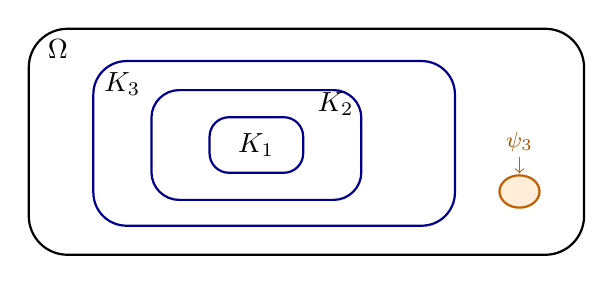
\begin{tikzpicture}[scale=0.82]
 \draw[thick,rounded corners=14pt] (-4,-1.7) rectangle (4.6,1.8);
 \draw[thick,rounded corners=12pt,blue!55!black] (-3.0,-1.25) rectangle (2.6,1.3);
 \draw[thick,rounded corners=10pt,blue!55!black] (-2.1,-0.85) rectangle (1.15,0.85);
 \draw[thick,rounded corners=7pt,blue!55!black] (-1.2,-0.43) rectangle (0.25,0.43);
 \node at (-0.48,0) {$K_1$};
 \node at (0.75,0.64) {$K_2$};
 \node at (-2.55,0.94) {$K_3$};
 \node at (-3.55,1.49) {$\Omega$};
 \draw[orange!75!black,thick,fill=orange!15] (3.60,-0.72) ellipse (0.31 and 0.25);
 \node[orange!65!black,font=\footnotesize] at (3.60,0.05) {$\supp\psi_3$};
 \draw[orange!75!black,->] (3.60,-0.18) -- (3.60,-0.44);
\end{tikzpicture}

\small\emph{Schemat:} funkcje testowe mogą mieć nośniki poza
kolejnymi zbiorami zwartymi, a wtedy nie tworzą ciągu zbieżnego
w topologii $\mathcal D(\Omega)$, nawet jeśli zbiegają do zera
w $C^\infty(\Omega)$.
\end{center}

\begin{uwaga}[Przejście do dystrybucji]
\label{rem:D-distributions-next18}
W kolejnym rozdziale zdefiniujemy przestrzeń dystrybucji
$\mathcal D'(\Omega)$ jako przestrzeń dualną topologiczną
$\mathcal D(\Omega)$. Podstawowe oszacowania funkcjonałów
uzyskaliśmy już w Uwadze~\ref{rem:D-dual18}; będziemy też
odróżniać topologię słabą-* od topologii zbieżności
jednostajnej na zbiorach ograniczonych funkcji testowych.
\end{uwaga}

% Materiał z AF 25; fragment do rozdziału o funkcjach testowych.
\subsection{Porównanie topologii przestrzeni funkcji testowych}
\label{sec:synteza25}

\begin{definicja}[Notacja porównawcza przestrzeni funkcji]
\label{def:trzy-przestrzenie25}
Zachowujemy przestrzenie $\mathcal E(\Omega)=C^\infty(\Omega)$,
$\mathcal D_K(\Omega)$, $\mathcal D(\Omega)$ i $\mathcal S(\R^d)$
z definicji \ref{def:DK18}, \ref{def:D-LF18}
oraz \ref{def:schwartz17}. Na $\mathcal E$ i $\mathcal D_K$
używamy seminorm
$p_{K,m}(f)=\max_{|\alpha|\le m}\sup_{x\in K}|\partial^\alpha f(x)|$.
Na $\mathcal S$ zapis $p_{N,m}(f)$ oznacza normę
$Q_{N,m}(f)$ z definicji \ref{def:schwartz17}.
Przestrzenie sprzężone topologicznie oznaczamy przez
$\mathcal E'$, $\mathcal D'$ i $\mathcal S'$; indeksy
$\sigma(X',X)$ i $\beta(X',X)$ oznaczają odpowiednio
topologię słabą-* (zbieżność punktowa na $X$)
i silną (zbieżność jednostajna na zbiorach ograniczonych).
Wszystkie przestrzenie rozpatrujemy nad wspólnym ciałem $\K$.
\end{definicja}

\begin{twierdzenie}[Ciągłe i gęste zanurzenia]
\label{thm:zanurzenia25}
Niech $d\ge1$. Odwzorowania identycznościowe
\[
 \mathcal D(\R^d)\longrightarrow\mathcal S(\R^d)
 \longrightarrow\mathcal E(\R^d)
\]
są ciągłymi, różnowartościowymi odwzorowaniami liniowymi o gęstych
obrazach. Dla dowolnego niepustego zbioru otwartego $\Omega\subseteq\R^d$
takie samo stwierdzenie zachodzi dla zanurzenia
$\mathcal D(\Omega)\to\mathcal E(\Omega)$.
Żadne z trzech wskazanych odwzorowań nie jest
izomorfizmem liniowo-topologicznym na swój obraz z topologią
podprzestrzeni; ostatnie stwierdzenie zachodzi dla każdego
niepustego zbioru otwartego $\Omega$.
\end{twierdzenie}
\begin{proof}
Dla ustalonego zwartego $K\Subset\R^d$ oraz $N,m\in\N_0$
mamy $p_{N,m}(f)\le (1+\sup_{x\in K}|x|)^N p_{K,m}(f)$
dla $f\in\mathcal D_K(\R^d)$. Stąd ciągłość
$\mathcal D_K\to\mathcal S$; własność uniwersalna granicy
induktywnej daje ciągłość $\mathcal D\to\mathcal S$.
Ciągłość $\mathcal S\to\mathcal E$ wynika z oszacowania
$p_{K,m}(f)\le p_{0,m}(f)$. Analogicznie sprawdzamy
ciągłość $\mathcal D(\Omega)\to\mathcal E(\Omega)$.

Aby wykazać gęstość, wybierzmy $\chi\in\mathcal D(\R^d)$
równe $1$ na kuli jednostkowej i zdefiniujmy
$\chi_R(x)=\chi(x/R)$ dla $R\ge1$. Dla $f\in\mathcal S(\R^d)$ i $|\alpha|\le m$
wzór Leibniza daje
\[
 \partial^\alpha((1-\chi_R)f)
 =\sum_{\gamma\le\alpha}\binom{\alpha}{\gamma}
 \partial^\gamma(1-\chi_R)\partial^{\alpha-\gamma}f.
\]
Wszystkie czynniki $\partial^\gamma(1-\chi_R)$
znikają dla $|x|<R$. Dla $\gamma\ne0$ są ograniczone
przez $R^{-|\gamma|}\sup|\partial^\gamma\chi|$,
a dla $\gamma=0$ przez $1+\sup|\chi|$.
Ponieważ $R\ge1$ i $(1+|x|)^{-1}\le(1+R)^{-1}$
na pozostałej części przestrzeni, otrzymujemy
\[
 p_{N,m}((1-\chi_R)f)
 \le \frac{C_{\chi,m}}{1+R}p_{N+1,m}(f).
\]
Zatem $\chi_Rf\to f$ w $\mathcal S$ i $\chi_Rf\in\mathcal D$.
Dla $f\in\mathcal E(\R^d)$ mamy $\chi_Rf=f$ w otoczeniu
każdego ustalonego zbioru zwartego przy dostatecznie dużym $R$,
a więc $\chi_Rf\to f$ w $\mathcal E$. W ogólnej
$\Omega$ używamy funkcji odcięcia $\chi_j\in\mathcal D(\Omega)$,
równej $1$ w otoczeniu $K_j$, gdzie $(K_j)$ jest
wyczerpaniem $\Omega$ zbiorami zwartymi. Każdy zwarty $L\Subset\Omega$ mieści się w pewnym $K_J$,
więc dla $j\ge J$ wszystkie pochodne różnicy znikają na $L$.
Stąd $\chi_j f\to f$ w $\mathcal E(\Omega)$.

Na $\R^d$ niech $\psi\in\mathcal D(\R^d)$ będzie niezerowa
i $f_n(x)=\psi(x-ne_1)$. Wówczas $f_n\to0$ w
$\mathcal E(\R^d)$, bo nośniki ostatecznie omijają każdy
ustalony zbiór zwarty, ale nie w $\mathcal S(\R^d)$,
gdyż $p_{0,0}(f_n)=p_{0,0}(\psi)>0$.
Z kolei $g_n(x)=e^{-n^2}\psi(x-ne_1)$ zbiega do zera w
$\mathcal S(\R^d)$: dla $\supp\psi\subseteq\overline B(0,A)$
mamy
\[
 p_{N,m}(g_n)\le e^{-n^2}(1+n+A)^N p_{0,m}(\psi)
 \longrightarrow0.
\]
Nie zbiega do zera w $\mathcal D(\R^d)$, gdyż nośniki
nie mieszczą się w jednym zbiorze zwartym
(Twierdzenie~\ref{thm:D-sequences18}).

Dla dowolnego niepustego otwartego $\Omega\subseteq\R^d$
wybieramy wyczerpanie $(K_j)$ jak w definicji.
Zbiór $\Omega\setminus K_j$ jest niepusty i otwarty,
bo żaden niepusty otwarty podzbiór $\R^d$ nie jest zwarty.
Wybieramy niezerowe $h_j\in\mathcal D(\Omega)$ takie,
że $\supp h_j\subseteq\Omega\setminus K_j$.
Wówczas $h_j\to0$ w $\mathcal E(\Omega)$, gdyż dla
każdego zwartego $L\Subset\Omega$ nośniki ostatecznie
omijają jego otoczenie (wybieramy $L\subseteq\operatorname{int}K_J$).
Gdyby $h_j\to0$ w $\mathcal D(\Omega)$, wszystkie nośniki
byłyby zawarte w pewnym zwartym $L\Subset\Omega$,
a więc w pewnym $K_J$. Dla $j\ge J$ oznaczałoby to
$h_j=0$, sprzecznie z wyborem. Topologia $\mathcal D(\Omega)$
jest zatem ściśle silniejsza od odziedziczonej z $\mathcal E(\Omega)$.
\end{proof}
